\chapter{Reconstructing the 2015 flash flood event of Salgar, the case of a poor gauged basin}\label{chap:4}
\footnotemark[1],\footnotemark[2]{\textit{Nicolás Velásquez}},
\footnotemark[1],\footnotemark[2]{\textit{Carlos D. Hoyos},
\footnotemark[1]{\textit{Jaime I. Vélez}},
\footnotemark[1],\footnotemark[2]{\textit{Esneider Zapata}},
\\

\footnotetext[1]{\textit{Geosciences and Environment Department, National University of Colombia - Medellín headquater}}
\footnotetext[2]{\textit{Sistema de Alerta Temprana del Valle de Aburrá (SIATA)}}

\textbf{Abstract.}
Flash floods events associated with severe precipitation events are highly destructive, often resulting in significant human and economic losses. Due to their nature, flash floods tend to occur in medium to small basins located within complex high mountainous regions. In the Colombian Andean region these basins are common, with the aggravating factor that the vulnerability is considerably high as some of these basins contain important human settlements. Settlements are frequently occupying floodplains and other flash-flood prone areas.  During  May 18 of 2015, two severe rainfall events generated a flash flood event in the municipality of Salgar, in the Liboriana basin located in the northwestern Colombian Andes, resulting in more than 100 human casualties and significant economic losses. The present work is a reconstruction of the hydrological processes that took place before and during the Liboriana flash flood event, analyzed as a case of a poorly instrumented basin.  The event conditions were recreated based on radar retrievals and a hydrological distributed model, linked with a proposed 1D hydraulic model and a shallow landslide model. Results suggest that the occurrence of two successive severe storm events cause the flash flood. Despite its simplicity, the proposed hydraulic model achieves a good representation of the flooded area during the event, with limitations due to the available spatial scale of the DEM (12.7 meters, from ALOS PALSAR images). From satellite images, we extract polygons observed landslides. For this case, the model simulates the landslide occurrence regions skillfully with small differences in the exact locations. To understand this case, radar data shows to be key due to specific convective cores location and rainfall intensity estimation. In mountainous regions, there exists a significant number of settlements with similar vulnerability, and with the same gauging conditions. The uses of low-cost modeling strategy could represent a good risk management tool in these regions with low planning capabilities.

%%-----------------------------------------------------------
%%-----------------------------------------------------------
%Introduction
%%-----------------------------------------------------------
%%-----------------------------------------------------------
\section{Introduction}  %% \introduction[modified heading if necessary]

\begin{figure}[t]
    \centering
    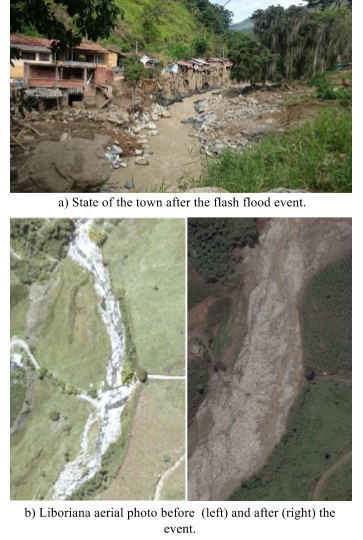
\includegraphics[width=8.3cm]{figuras/Figura1_Antes_y_despues.png}
    \caption{Affections after the flash flood occurred May 18 of 2015. a) State of some houses near the entrance of Liboriana river to Salgar urban area. b) comparison of Liboriana river delineation before and after the event.}
    \label{fig:Antes_y_Despues}
\end{figure}

Usually, flash floods are described as rapid events related to convective rain systems \citep{Salek2006,Llasat2016,Douinot2016}. Considered one of the most destructive hydrological hazards \citep{Roux2011}, that could represent high costs related to human and infrastructure losses. Additionally, to intense rainfalls, several studies show that antecedent soil moisture influence flash floods \citep{Tramblay2012b,Rodriguez2012,Coustau2012,Wagener2007,Castillo2003}. There is too, an influence due to hills and stream slopes \citep{Doswell2001,Salek2006}, being apparently more important the slopes at the hills \citep{Roux2011,Yatheendradas2008}. Due to flash floods rapid response, and related high changes at the streamflow, they are usually analyzed at detailed temporal scales \citep{Norbiato2008} in smalls basins \citep{Younis2008}.  This conditions difficult their predictions \citep{Hardy2016,Ruiz-Villanueva2013} and increase related uncertainties \citep{Wagener2007}.\\ 

There are plenty of studies that analyze and reconstruct flash floods, with different views.  Some do it from a climatological approximation, \citet{Piper2016} examine the key features of the storm statistically, \citet{Fragoso2012} analyze storm characteristics and required rainfall conditions. \citet{Aronica2012} using GIS and statistical estimates, investigate the hydrological and climatological conditions and reconstruct associated landslides and depositions.   Other authors try to understand the governing processes of flash floods, \citet{Vannier2016} analyze the role of the geology in the south of France. \citet{Adamovic2016} use a simple model to simulate flash floods and explain the associated process. \\ 

The use of radar data could overcome the lack of precipitation data at small basins \citep{Creutin2003}, nowadays the use of radar-derived data is becoming more common to analyze flash flood events \citep{Salek2006,Garambois2015}.  Radar data is being used too into flash floods forecast, \citet{Hardy2016} presents an application of a probabilistic ensemble over the US, and \citet{Ravazzani2016} compare two ensembles over Milano.  In general, there is an optimistic future for flash flood understanding taking into account the actual radar and rain gauge data\citep{Braud2016}.\\   

As mentioned before, flash floods tend to happen at mountainous regions, with steep slopes. Also, usually detonated by the occurrence of convective storms events. This type of rainfall features high intensities, low durations, and a relatively small spatial coverage.  An essential portion of the Andean region at Colombia fulfills the described conditions; orographic conditions increase convective cores occurrence \citep{Poveda2007}. Additionally, hills exhibit crucial elevation differences with associated steep slopes. The ITCZ overpass rise the probabilities of flash floods occurrence, this due to an increase of convective cores presence.\\   

Between May 15 and May 18, several storm events took place over the Liboriana basin. During the night of 17 of May, a stratiform formation covers almost all the basin, 20 hours later (May 18) multiple convective cores happen in the upper region of the basin.  We think that the described rainfall can explain the flash flood that took place after the midnight of May 17, this event took about 100 lives and affected buildings and infrastructure.\\   

The described event presents essential soil moisture antecedent conditions related. On May 17 at 5:00 A.M, a storm with a significant rainfall accumulation (47 $mm$) happen at the basin (named for this work as event 1).  Additionally, just before the principal storm, at 11:00 P.M on May 17, happens a previous event in the same basin region (beginning of event 2).  Event 1 is characterized mainly as stratiform, covering almost all the basin area.  On the other hand, event 2 is composed of multiple convective impulses, happening in the upper part of the basin. Event 1 increase overall soil moisture with an associated decrease on infiltration rates \citep{Penna2011,Zehe2010}, low infiltration increase runoff rates, which finally affects the vulnerability of the basin against flash floods occurrence \citep{Wagner1999,Penna2011,Tramblay2012b}. \\

Liboriana basin is a case of Prediction in Ungauged Basins (PUB) \cite{Sivapalan2013, Seibert2009, Beven2007, Bonell2006}, this regarding flash floods.  There are no hydro-meteorological records, soils, and land use maps; we obtain information from satellite data, field visits, and radar rainfall estimations.  Due to this lack of data, Liboriana case imposes a challenge for flash flood prediction and modeling \citep{Sivapalan2013,Yamanaka2017}.  According to \citet{blschl2012} there are three methods to calibrate models for PUB cases: 1) obtain parameters from apriori characteristics, which could lead to low-performance \citep{Duan2006}, 2) inherit calibration from a near basin, which in this case doesn't exist, and 3) calibrate based on proxy variables, such as hydraulic information obtained during field recognition.  There are no old streamflow records from Liboriana basin, or records from a neighbor basin, because of this, option 3 seems to be likely to be used for Liboriana case.\\

In the case of the flash flood of Salgar the authors want to explore two main ideas. The first notion consists in analyzing the relationship between rainfall structure \citep{Llasat2016,Fragoso2012}, soil moisture and runoff generation \citep{Penna2011,Tramblay2012b,Garambois2013}.  The second idea consists in a modeling approximation to the hydrological and natural hazard processes that took place. With the objective of present a low-cost tool that could be used for local early warning systems or as a planning tool.\\   

For the first idea, we reconstruct and validate the hydrological processes.  For the modeling process, we use a self-edited version of the SHIA model \citep{Frances2007b}, the WMF model. It is a conceptual distributed hydrological model that separates hydrological process as storages.  A calibration of the model is done based on field information of a cross section located at the entrance of the urban area of Salgar. Additionally, we analyze hydrological processes with the storage states of the model. Also, putting virtual traces in the model that separates runoff from the sub-superficial flow.  Processes analysis is completed comparing hydrological results with rainfall variability, for this, we split rainfall into convective and stratiform \citep{Houze2015,Steiner1995}. The model marks classified rain and follows it along the network.  Interactions between runoff, sub-superficial flow, and convective-stratiform rainfall give a better hydrological understanding.\\

We analyze natural risks using the hydrological modeling results. For this, we use two sub-models.  A Shallow landslides model \citep{Aristizabal2016} is attached to the hydrological model. And for flash flood, we propose a 1D hydraulic model (\textbf{HydroFlash}). It is a low-cost model that assumes infinite sediment supply, and estimates filled area at each cross section. We compare results from both sub-models with observed affections (landslides scars and flood spots). For the comparison, we use satellite photos taken days after the event (Google, Landsat/Copernicus).  According to obtained results, it is possible to use these low cost models as a risk management tools in countries and places with scarce resources.\\  

Present work is structured as follows: 1) data and Liboriana zone basin description, geomorphological and climatological characteristics of the basin are presented, along with the information used. 2) Description of the models and the methodology, including fluxes separation, shallow landslides, and the proposed hydraulic model. 3) Presentation of results and discussions, it includes calibration and validation process. Here we discuss the role of the rainfall structure and present results from sub-models. 4) Finally, are the conclusions, we consider the possibility to implement this kind of models in places with scarce information.\\

%%-----------------------------------------------------------
%%-----------------------------------------------------------
%Information
%%-----------------------------------------------------------
%%-----------------------------------------------------------
\section{Data and Zone Description}


The town of Salgar is near the outlet of the Liboriana basin. It is a small tropical basin (56$km^2$) that starts at the Cerro Plateado mountain, located in the occidental mountain range of Colombia (Figure \ref{fig:Ubicacion}). At its outlet, Liboriana joins the Barroso river, then both drain to the Cauca river.  The highest portion reaches 3600 meters above sea level, and the outlet is at 1300 meters (see Table \ref{tab:geomorfologia}), longitudinal profile (colored line in Figure \ref{fig:Perfil}) exhibit significant steeps slopes in the upper region.  Hypsometric curve presents considerable elevation changes for cumulated areas below 33\% of the total area (blue line at Figure \ref{fig:Perfil}).  Described geomorphological characteristics are typical of Andean mountainous basins. Usually, this kind of watersheds is prone to flash floods events occurrence.   The trace of the basin for modeling and geomorphological analysis was done using an ALOS-PALSAR Digital Elevation Model (DEM) \citep{ALOS}, with a spatial resolution of about 12.7$m$.\\

\begin{table}[t]
  \caption{Geomorphological parameters of Liboriana basin.}
  \begin{tabular}{lr}
  \hline
    \textbf{Parameter} & \textbf{Value} \\    
  \hline
    \textbf{Basin parameters} & \\
    Basin Area $[km^2]$ & 56.8\\
    Perimeter $[km]$ & 57.8\\
    Mean Slope $[\%]$ & 57.6\\
    Basin Longitude [$km$] & 13.5\\
    Maximum elevation $[m]$ & 3609\\
    Minimum elevation $[m]$ & 1316\\
  \hline
      \textbf{Network Parameters} & \\
      Strhaler Horton Order & 4\\
    Principal Stream longitude [$km$] & 18.1\\
    Principal Stream slope [$\%$] & 8.1\\
  \hline
  \end{tabular}
  %\belowtable{Geomorphological properties of the basin where calculated in automated way using the WMF model, and could be estimations of the real parameters values.} % Table Footnotes
  \label{tab:geomorfologia}
\end{table}

At sub-basin scale, Liboriana basin presents different slopes and height differences.  Figure \ref{fig:Ubicacion} presents the HAND model (Height Above the Nearest Drainage)  \citep{Renno2008}. HAND calculates the relative difference between cell $i$ and its nearest destination streamflow cell $j$.  According to HAND,  differences reach values between 500 and 800$m$. Near the outlet, in the banks, there are values near 0 meters.  High HAND values at the upper region increase potential energy, with increased sediment production and shallow landslides occurrence.  On the other hand banks with low HAND values are more vulnerable to flash floods, and tend to present extensive affected areas in the valley.  Elevation differences described are typical of the region, here the problem lies in the urban area localization at the outlet.\\ 

\begin{figure}[t]
\centering
    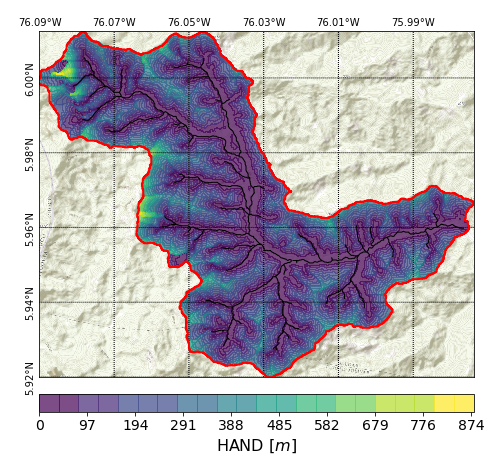
\includegraphics[width=8.3cm]{figuras/HAND_Ubicacion.png}
    \caption{Liboriana basin localization in Colombia and Antioquia.  Color bar represent the Height Above the Nearest Drainage (HAND), low values correspond to areas prone to inundations, high values .}
    \label{fig:Ubicacion}
\end{figure}
\begin{figure}[t]
\centering
    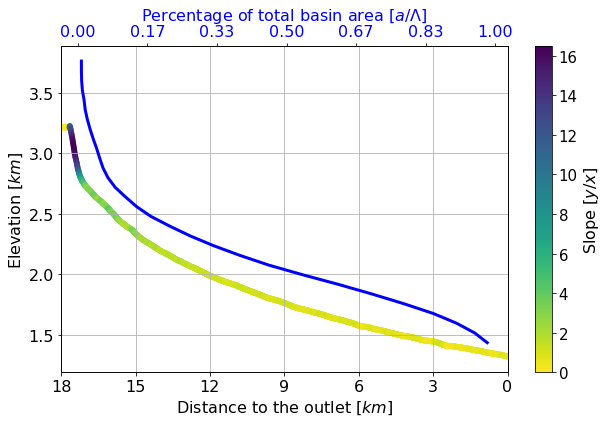
\includegraphics[width=8.3cm]{figuras/Perfil_Cauce.png}
    \caption{Mean stream longitudinal profile (changing color line) from the upper part of the basin to its outlet at the entrance of the urban area, and mean basin hipsometric curve (blue line).}
    \label{fig:Perfil}
\end{figure}

Land use and vegetation vary in the basin. In the upper region there are crop fields and tropical forests, also, a portion of it is considered a national park.  Hills near the boundary line of the basin do not present significant human interference, this in part due to the steep slopes in this region.  Down the hills, at the bottom of the valley there is presence of coffee crops and pastures, also, near the banks there are grazing areas and urban development.\\

Andean Colombian region tends to present well developed various soils textures, with an essential presence of limes and clays at some areas.  Soils in the region are not well mapped; national soil cartography usually is presented in a scale of 1:400.000, at this scale the county of Salgar and Liboriana basin corresponds to one soil texture. For this case there are only descriptions given by regional authorities and geologists, \citet{Osorio2008} describes the soils as well-drained, with poor retentions capacity. The organic material covers the first layer; a second layer is covered by a clay loam soil also well-drained.  The depth of the soils is assumed to be hill slope dependent, varying between 20$cm$ and 1$m$ \citep{Osorio2008}. Table \ref{tab:suelos} resume soils into five classes according to the slope. Each soil feature has an assigned depth and a qualitative description of permeability and retention.\\

\begin{table}[t]
  \caption{Soils description given by the IGAC institute.}
  \begin{tabular}{lcccr}
  \hline
    \textbf{Type} & \textbf{Slope} & \textbf{Depth [$m$]} & \textbf{Retention} & \textbf{Permeability} \\    
  \hline
    \textbf{Class III} & 12-25 & 0.6 & Mean & Mean \\
    \textbf{Class IV} & <12 & 0.6 & Low & High \\
    \textbf{Class VI} & 25-30 & 1.0 & Mean & Mean \\
    \textbf{Class VII} & 30-50 & 0.3 & Too Low & Slow \\
    \textbf{Class VIII} & >50 & 0.2 & Too Low & Slow \\
  \hline
  \end{tabular}
%   \belowtable{The description given by the IGAC institute is subjective, without mentioning exact values of retention and permeability.  The depth values given are approximations.} % Table Footnotes
  \label{tab:suelos}
\end{table}

To obtain a reference point for the model calibration, we did a field campaign days after the flash flood event.  We made a visual inspection of the principal stream and flood spots. During this fieldwork, we obtain the section at the entrance of the urban area, located at the outlet of the basin (Figure \ref{fig:Ubicacion}).  The cross-section has a rectangular shape, with 4.6$m$ width and 5$m$ height, it has an area of about 23$m^2$.  At the place, buildings exhibit mud marks varying between 0.5 and 1.2 $m$, with horizontal distances from the channel of 4 and 5 $m$.  Sectional area plus the flooded area is estimated to be equal to 37$m^2$.  Assuming flow speeds between 3 and 6 $m/s$, the streamflow required to produce a flood could vary between 111 and 222 $m^3/s$.  We validate our results with this estimated values and the satellite images.\\ 

Precipitation data is obtained by a meteorological radar located at 100$km$.  Radar data is acquired and processed by the Sistema de Alertas Tempranas de Medellín y del Valle de Aburra (SIATA), a local early warning system from a neighbor region.  The radar is a band C polarimetric Doppler radar,  with a maximum operating range that oscillates between 200 and 500 $km$, and an optimum range of 120 $km$.  Data acquisition is made with a time step of 5$min$.  Operational specifications and radar characteristics let us work rainfall at a resolution of 128 $m$.  \\

%%-----------------------------------------------------------
%%-----------------------------------------------------------
%Methodology
%%-----------------------------------------------------------
%%-----------------------------------------------------------
\section{Methodology}

For this work, we rewrite the SHIA model \citep{Frances2007b}.   The model includes essential modifications and is packed under the Watershed Modelling Framework \textbf{WMF} (allocated in a web repository: \href{https://github.com/nicolas998/WMF.git}{\textbf{GitHub}} ).  Modifications include the set of a maximum gravitational storage ($H_{g}$), the opening of equations, open rain field usage, flux separation at the streamflow and rainfall type (convective, stratiform) separation in the basin.  Additionally, we include two modules for hazard estimation: a shallow landslide model \citep{Aristizabal2016}, and a new low-cost 1d hydraulic flash flood model named \textbf{HydroFlash}.  The hydrological model and sub-models are written in Fortran 90, interface to the model, pre-process and post-process tools are in python 2.7, Fortran code is warped to python using \textbf{f2py} \citep{Peterson2009}.  For the classification of convective and stratiform formations, we use the algorithm of \citet{Steiner1995}. Reflectivity to rainfall transformation uses land rainfall measurements and disdrometer data.\\  

\subsection{Hydrological model modifications}

The Hydrological model has four main modifications.  The model could use rainfall fields from any source of information; this includes interpolated and radar data.  In the other hand, tank 3 (gravitational storage) now has a limit storage ($H_g$). Horizontal flux equations could be linear or potential, as shown in equation (\ref{eq:generica}).  In the new model concept, $\beta$ and $\alpha$ are estimated by the user and then given to the model. Finally, the model includes virtual tracers.  One to separate runoff from sub superficial flow.  The other to track convective and stratiform portions of the stream.\\  

\begin{equation}
 v_{tank}(t) = \beta A(t) ^{\alpha}
    \label{eq:generica}
\end{equation}

Non-linear equations in lateral flux could give a better representation of processes at high resolutions \citep{Beven1981}. Being more explicit in runoff processes, and sub superficial flow processes \citep{Beven1981, Kirkby1967}.  A non-linear approximation to runoff is presented in equation (\ref{eq:runoff}).   It is a modification of manning's formula for flux in gullies, in the equation according to \citep{Foster1984}, the values of $\varepsilon$ and $e_1$ are 0.5 and 0.64 respectively.   Equation (\ref{eq:kubota}) presents the non-linear approximation for sub superficial flow,  it is an adaptation of \citet{Kubota1995} formula. In which $k_s$ is the saturated hydraulic conductivity, and $b$ is dependent on the soil type, assumed equal to 2.  $A_g$ is the equivalent cross-section area to the maximum gravitational storage ($H_g$). \\

\begin{equation}
 v_{2} = \frac{\varepsilon}{n}  S_{0}^{1/2} A_{2}(t)^{(2/3) e_1}
    \label{eq:runoff}
\end{equation}
\begin{equation}
 v_3 = \frac{K_s S_{o}^{2}}{(b+1) A_{g}^{b}} A_{3}(t)^{b}
    \label{eq:kubota}
\end{equation}

Described equations describe the momentum of a kinematic wave approximation. In both cases speed is related to the tank storage (or sectional area). This relations could be resumed by the equation (\ref{eq:generica}),  that numerically could be solved coupled with a mass balance equation (\ref{eq:balance}). This equation takes into account the storage at each time step ($S_{tank}(t)$), the longitude of the element ($\Delta x$), the time step size ($\Delta t$), and the speed estimated for the flux in the time step ($v_{tank}(t)$).  Equation (\ref{eq:balance}) is related to equation (\ref{eq:generica}) through the speed term ($v_{tank}$) and the sectional area ($A$).  The solution to $v_{tank}$ and $A$ is obtained through an iteration scheme, in order to ensure numerical convergence, the initial values for $v_{tank}$ are assumed equal to 0.5. And for the next iterations $v_{tank}$ takes as initial value the one estimated in the last time step ($v_{tank}(t) = v_{tank}(t-1)$).  Total out flux from the tank is calculated using equation (\ref{eq:volSalida}), this when $v_{tank}$ and $A$ are estimated.  Remaining model processes explanation could be found at \citet{Frances2007b}.\\

\begin{equation}
 A(t) = \frac{S_{tank}(t)}{\Delta x + v_{tank}(t) \Delta t}
    \label{eq:balance}
\end{equation}
\begin{equation}
    E_{tank}(t) =  A(t) v_{tank}(t) \Delta t
     \label{eq:volSalida}
\end{equation}

\subsection{Virtual Tracers}

We add two virtual tracers to the model.  One is a flux tracer that separates the streamflow into runoff and sub superficial flow, recording at each time step and each element the origin of water. The other is a rainfall type tracer that separates streamflow into its convective and stratiform rainfall portions, in this case, it separates rain from the rainfall inputs.  The tracer records results at the outlet of the basin and at each reach; this let us get an idea of how the interactions of fluxes vary across different scales.\\

\subsubsection{Runoff and Sub-superficial Separation}

With the flux separation, we pretend to get more insights about the role of the soil and get an idea of how is the relation between the runoff and sub superficial flow.  The texture and the composition of the soil could play different roles in this event; it could work as a porous medium in which the water travels fast, making the sub-superficial flow an essential part of the hydrograph.  On the other hand, it's saturation could lead to a decrease in infiltration rates and a possible increase of runoff generation.\\

The flux separation module operates over tanks 2 (runoff storage) and 3 (sub-superficial storage).  It marks water once it reaches any of those two tanks, the percentages of participation are taken into account when this water goes into the channel (tank 5).   At this point, the separation scheme assumes that the channel storage flows homogeneously,  this assumption implies that fluxes participation is constant until a new inflow comes into the channel.  Here is an example of how the separation works: suppose tank five has 100$[mm]$ in cell $i$ ($S_{5,i}$), 60$mm$ correspond to runoff, 35 to sub superficial and 5 to baseflow.  If at time $t+\Delta t$ the outgoing flow is $E_{i,5} = 95[mm]$, outgoing runoff and sub superficial flow will be respectively $Erun_{i,5} = 0.6 E_{i,5}$ and $Esub_{i,5} = 0.35E_{i,5}$.\\     

\subsubsection{Convective and Stratiform Tracers}

Both spatial and temporal rainfall variability influence the hydrograph formation, this rainfall variability both in time and space is subject to the structure of the storm \citet{Shope2016}. Stratiform rain cells cover several areas and are related to long duration hydrographs with low peak flow.  On the other hand, convective rainfall cells cover less space and are related to short duration hydrographs with high peak flows.  Stratiform rainfall tends to recharge the basin, and convective tends to increase runoff generation and the formation of the hydrograph.  In the literature, these associations have been more qualitative than quantitative.\\

We classified rainfall before the usage of the rainfall tracer, convective and stratiform system classification is done from the radar reflectivity \citep{Steiner1995}. At each time step, the model reads classified rainfall; it assumes that the rain of a cell is convective or stratiform.  This assumption could lead to estimation errors at basins composed of coarse cells (high values of $\Delta x$). This because in elements with increased areas there are more chances of a convective-stratiform merge.  In the present study $\Delta x$ is equal to 12.7$m$, each cell element has an area of about 161$m^2$, at this spatial scale it is possible to make this assumption.  Once in the model, rain separation follows the methodology proposed for flux type separation. Convective and stratiform water is follow through tanks in each cell, each hydrological junction shows the results from the separation.\\

\subsection{Natural Hazards Simulations}

During the flash flood event of May 18, two central processes took place. Shallow landslides occurred in the upper part of the basin.  And related to landslides, a flash flood generates inundations, and human and infrastructure losses.  Coupled with the SHIALANDSLIDE and HydroFlash, the hydrological model simulates both events.  The models are presented and described.\\

\subsection{Shallow landslides sub-model}

Shallow land slides model coupled to the TETIS model is proposed and presented by  \citeauthor{Aristizabal2016}.  The model conceptualizes the stability of a cell with the concept of an "infinite slope." It assumes that this portion of the cell represents its geomorphological and soil properties. Figure \ref{fig:ModeloEstabilidad} describes the variables of the model and the balance of forces done.  

\begin{figure}[t]
\centering
 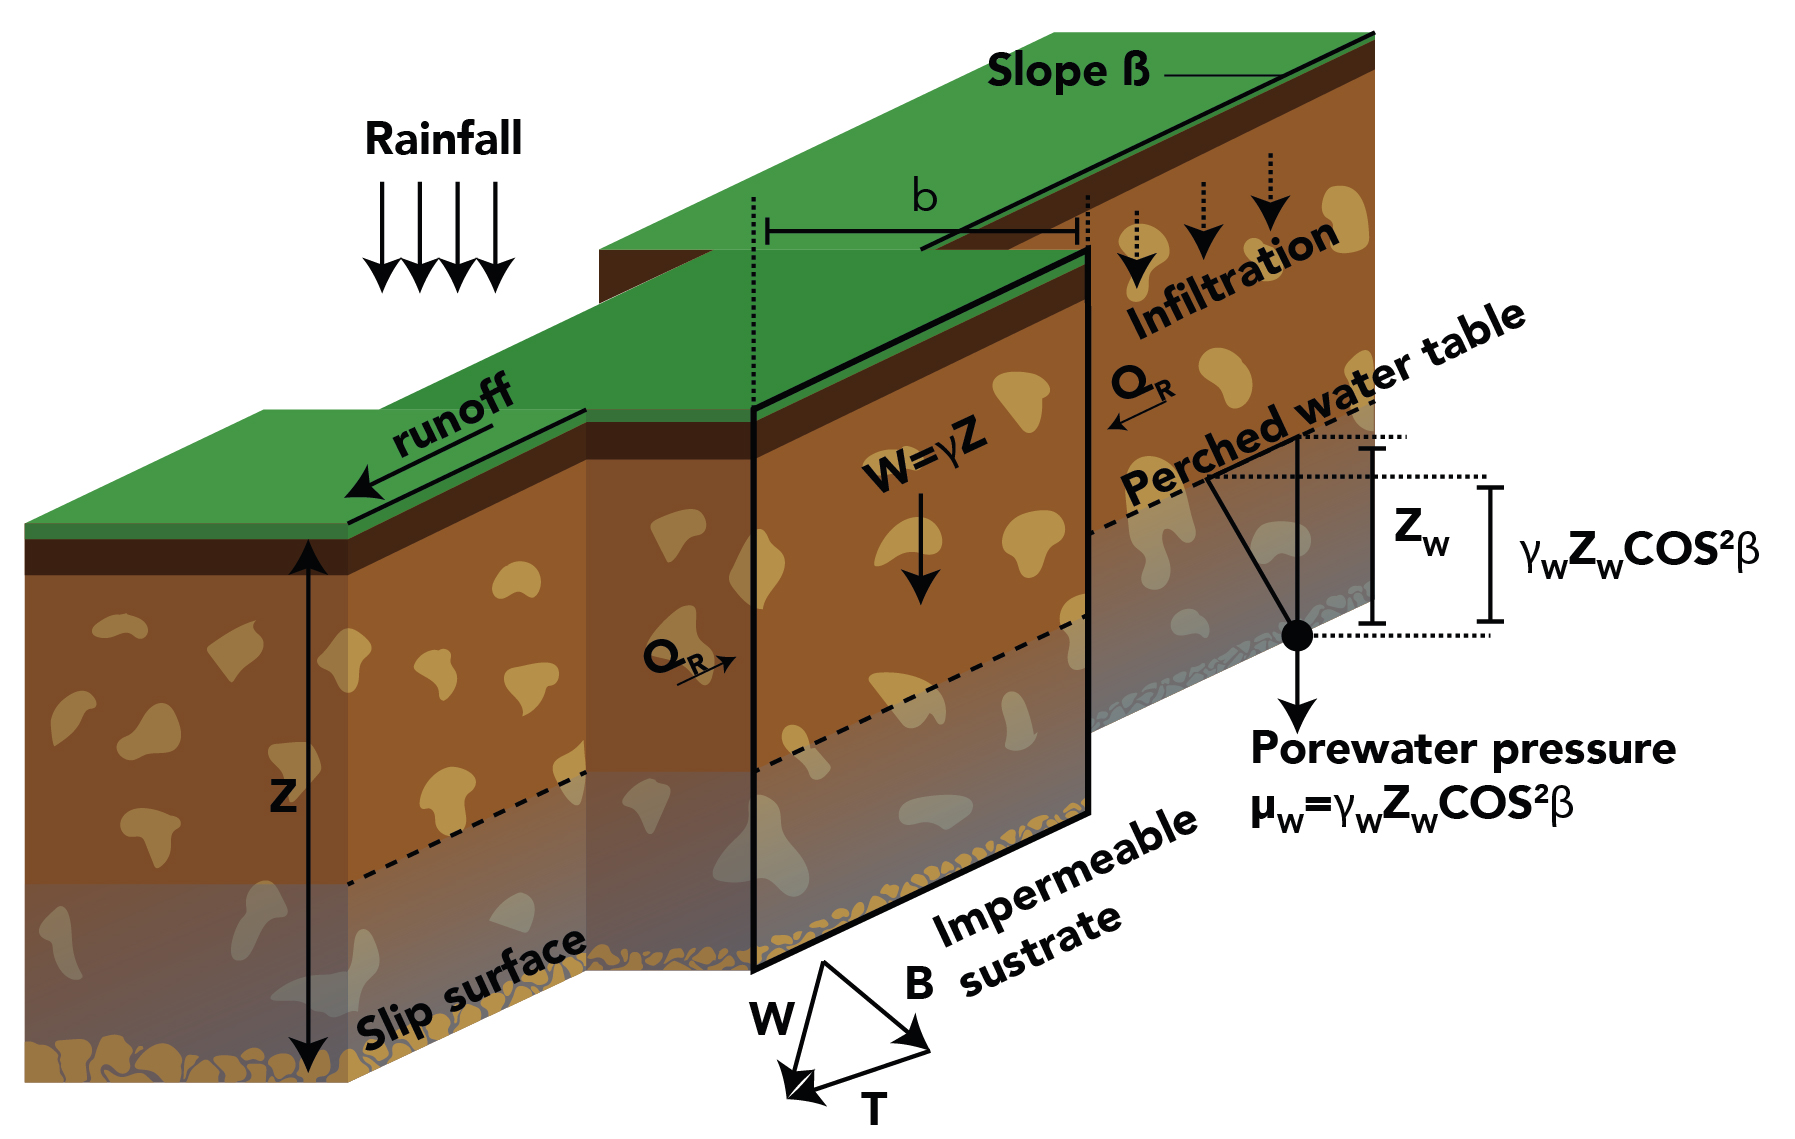
\includegraphics[width=8.3cm]{figuras/slides-escheme.jpg}
 \caption{The geotechnical conceptual model. $\gamma$ is the soil bulk density, $\gamma_w$ is the water density, $Z_w$ is the saturated soil thickness above the slip surface, $Z$ is the soil
thickness measured vertically, $\beta$ is the gradient of the hillslope. And $Q_L$ and $Q_R$ are the resultant forces on the sides of the slice.  Figure and description are adapted from \citet{Aristizabal2016}.}
    \label{fig:ModeloEstabilidad}
\end{figure}

The stability model classifies cells into three groups: unconditionally stable, conditionally stable and unconditionally unstable.  Three parameters determine the cell type.  Residual soil thickness water table $Z_{min}$ (equation (\ref{eq:zmin})).  The maximum soil depth at which a certain soil stills remains stable $Z_{max}$ (equation (\ref{eq:zmax})).  And the maximum slope value at which the portion of soil stills stable $\beta_0$ (equation (\ref{eq:bo})). \\

\begin{equation}
 Z_{i,min} = \frac{C^{'}}{\gamma_w cos^2 \beta tan \phi + \gamma cos^2 \beta (tan\beta - tan \phi)}
    \label{eq:zmin}
\end{equation}
\begin{equation}
 Z_{i,max} = \frac{C^{'}}{\gamma cos^2 \beta (tan\beta - tan \phi)}
 \label{eq:zmax}
\end{equation}
\begin{equation}
 \beta_{0,i} = tan ^{-1} \left[ tan \phi \left( 1- \frac{\gamma_w}{\gamma}\right) \right]
 \label{eq:bo}
\end{equation}

The model evals conditionally stable cells in function of their perched water table ($Z_{i,w}$) and the critical satured depth ($Z_{i,c}$).  With equation (\ref{eq:z}) the model calculates $Z_{w,i}$. In which $S_{3,i}$ represents gravitational storage, $Ws$ and $W_{fc}$ the soil saturation and field capacity respectively. Failure occur when $Z_{w,t}$ is greater than $Z_{i,c}$.  It obtains $Z_{i,c}$ from (equation (\ref{eq:Zcrit}), where $\gamma$ represents soil density, $\phi$ is the soil stability slope, and $\beta$ is the cell slope.  The model doesn't evaluate unconditionally stable and unstable cells during execution.\\

\begin{equation}
 Z_{w,i}(t) = \frac{S_{3,t}}{W_c - W_{fc}}
 \label{eq:z}
\end{equation}
\begin{equation}
 Z_{i,crit} = \frac{\gamma}{\gamma_w} Z \left( 1-\frac{tan \beta}{tan\phi} \right)
     + \frac{C^{'}}{\gamma_w cos^2 \beta tan\phi}
 \label{eq:Zcrit}
\end{equation}

\subsection{Flash flood hydraulic sub-model HydroFlash}

For flood spots simulation it is common to use complex hydraulic 2D and 3D models, such as Iber \citep{Cea2015} or HEC \citep{Gibson2010} .  This kind of modeling tends to involve detailed information about the terrain and river bathymetry.  People apply them to a river section, this due to high information demand and high computational costs.  High requirements of information preclude the usage of 2D and 3D methodologies in regions with scarce resources.  Additionally, operational implementation of these models carries technical issues. Such as increased computational demand. Also, this classical hydraulic approximation tends to analyze only some network elements. And leaves behind the complexity of the basin.\\

We introduce a low cost 1D hydraulic model for flash flood simulation HydroFlash.  It is a low-cost model that operates with the hydrological model. The model doesn't imply significant increases in execution time. The models extract from the DEM the cross-profile for each cell considered network.  It estimates flood spots at each network cell during execution time.\\

All network cells require certain hydraulic parameters for the model.  With equation (\ref{eq:ancho}) it estimates channel width ($w_i$).  And, it estimates channel slope ($S_{i,0}$) as the mean value of the slopes that correspond to the cells of a hydrological reach. Characteristic particle diameter $D_{i,50}$ is assumed equal to 0.138 and constant.  From the DEM the model obtains the cross-section ($C_s$). It extracts $C_s$ perpendicular to flow direction of the cell ($D_{i,8}$). For example, if a cell direction is \textbf{north}, $C_s$ takes elevation values from east to west of the cell. Except for $C_s$, described parameters correspond to each hydrological sections.\\

\begin{equation}
 W = 3.26 \overline{Q}^{0.469}
 \label{eq:ancho}
\end{equation}

At each time step $t$ and for each cell with stream, equation (\ref{eq:altura}) determines the height of the water table ($Y_{i}(t)$). This using simulated streamflow ($Q_{i,sim}$(t)) and speed ($v_{i,sim}(t)$). Then using $Y_i$ and equation (\ref{eq:velocidad}) the model calculates the friction speed ($v_{fr,i}$). This is derived from Keulegan and Rouse equations. Concentration ($c_{i}(t)$) and constitutive coefficient ($r_{i}$) are estimated using equations (\ref{eq:con}) and (\ref{eq:rdf}) respectively. The step is finished estimating the stream flow plus estimated sediments and rubble (equation (\ref{eq:qescombros}).\\

\begin{equation}
 Y_i = \frac{Q_{i,sim}}{v_{i,sim} w_{i}}
 \label{eq:altura}
\end{equation}
\begin{equation}
 v_{fr,i} = \frac{v_{i,sim}}{5.75 log \left( \frac{Y_{i}}{D_{i,50}} \right) + 6.25}
 \label{eq:velocidad}
\end{equation}
\begin{equation}
 c_{i} = C_{max} (0.06 Y_{i})^{\frac{0.2}{v_{fr,i}}}
 \label{eq:con}
\end{equation}
\begin{equation}
 r_{i} = \left( \frac{1}{D_{i,50}} \right) \left(  \left( \frac{9.81}{0.0128} (c_i + (1-c_i) \right)  \left( \frac{\gamma_w}{\gamma_{sed} }\right)   \right)^{0.5} \left( \frac{C_{max}}{c_i} \right)^{(1/3)-1.0}
 \label{eq:rdf}
\end{equation}
\begin{equation}
 Q_{i,sed} = Q_{i,sim} \frac{1+c_i}{1-c_i}
 \label{eq:qescombros}
\end{equation}
 
Assuming infinite sediment and rubble supply, $Q_{i,sed}$ is the maximum stream flow that could happen in the section.  To determine the flooded area, an equivalent $Y_{i,sed}$ must be found in order to obtain an stream flow ($\hat{Q}_{{i,sed}}$) (equation (\ref{eq:constitutiva})) that equals $Q_{i,sed}$.  The estimation of $Y_{i,sed}$ is an iterative process with small increasings of $\Delta y_{i,sed}$.  The model obtains the flooded area ($A_{i,sed}$) based on $Y_{i,sed}$ and equation (\ref{eq:differencia}).  The iteration stop when $\hat{Q}_{i,sed}$ reach a value near $Q_{i,sed}$.  At this point the model records flooded cells and flood depth.\\ 
 
 \begin{equation}
  \hat{A}_{i,sed} = \Delta x \sum_{j=1}^{N} (Y_{i,sed}+\Delta y_{i,sed}) - C_{j,s} 
  \label{eq:differencia}
 \end{equation}
 \begin{equation}
   \hat{Q}_{i,sed} = \left( \frac{2}{5} \right) r_i(j \Delta y_{i,sed})^{\frac{3}{2}} S_{i,0} 0.5 \hat{A}_{i,sed} 
 \label{eq:constitutiva} 
 \end{equation}

Resulting flooding maps tend to present two main issues.  The presence of small isolated flood spots. And discontinuities at flood spots when flow direction change from orthogonal to diagonal.  We include two post-process steps that correct described issues.  By the use of an erosion algorithm, we remove the small isolated flood spots. This erosion is done once and with a kernel of 3x3.  To solve diagonal discontinuities, each flooded cell seeks to flood its 8 neighbors.  A neighbor cell is flooded if the elevation of the flooded cell plus its flood depth is higher than its height.  The neighbor flood depth will be the difference of both elevations.\\ 
%%-----------------------------------------------------------
%%-----------------------------------------------------------
%Results
%%-----------------------------------------------------------
%%-----------------------------------------------------------
\section{Results and Discussion}

As mentioned in the introduction, we present results in two steps.  First, there are the results from simulation and the discussion of the related process. Second the re-creation of two natural hazards: shallow landslides, and flash floods.\\

\subsection{Calibration and Validation}

Figure \ref{fig:SimStreamflow}a presents hydrological simulation results at the outlet of the basin.  Base flow storage is set to achieve a base flow of 3 $m^3/s$, value that correspond to the observed value during the liquid reading.  According to the meteorological radar, one day before the event there was a rainfall event (17/05/2015).   The precedent event was higher than the one that produces the flash flood.   Developing an important hydrograph ($Q_{max} = 160 m^3/s$), that do not derive in casualties or losses.  Due to this, flash flood event happens under wet conditions (see the purple line in Figure \ref{fig:SimStreamflow}b).  Additionally, during the flash flood event happen two successive convective cores in the same region.   Simulation results suggest a peak flow of 225 $m^3/s$ (purple line Figure \ref{fig:SimStreamflow}a), value that surpasses field estimated limit streamflow (111-222 $m^3/s$).\\

\begin{figure}[t]
\centering
 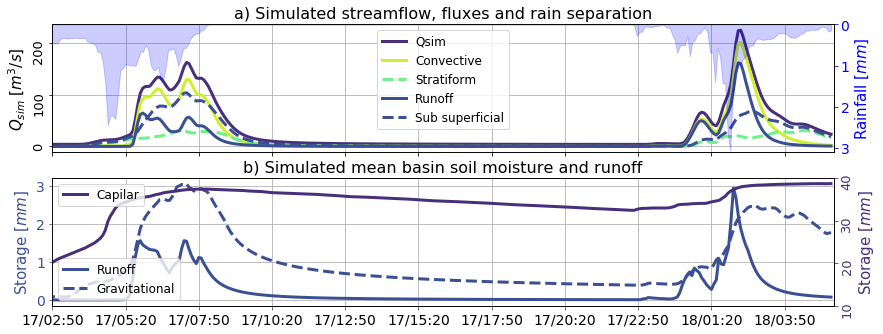
\includegraphics[width=8.3cm]{figuras/Caudal_Sim.png}
 \caption{Hydrological simulation results resume. a) Simulated streamflow, rainfall separation and runoff and sub-superficial flow separation. b) Mean runoff, gravitational, and capillary storages during the simulation period.}
    \label{fig:SimStreamflow}
\end{figure}

\begin{figure}[t]
\centering
 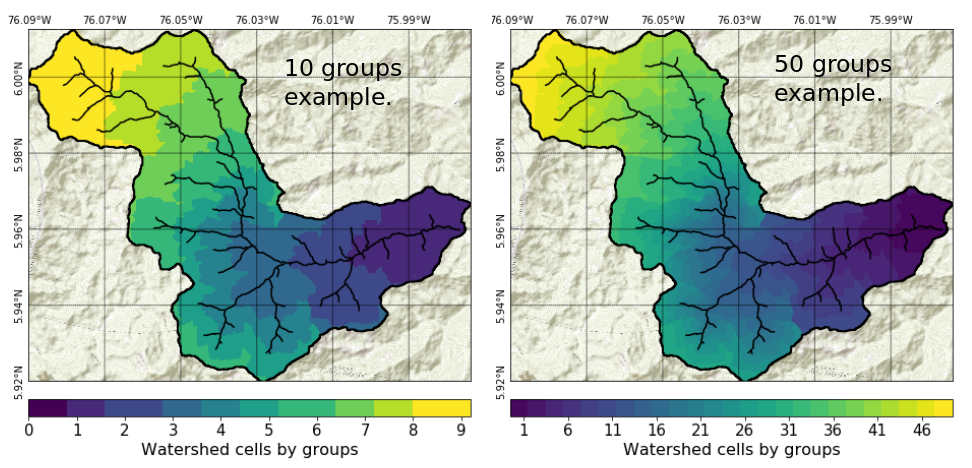
\includegraphics[width=8.3cm]{figuras/Mapas_Grupos.png}
 \caption{Graphical explanation of the groups that form the basin. Left image corresponds to an example of the basin split into ten different groups. Right image actual categorization of 50 groups.}
    \label{fig:ExplainationGroups}
\end{figure}

\begin{figure}[t!]
\centering
 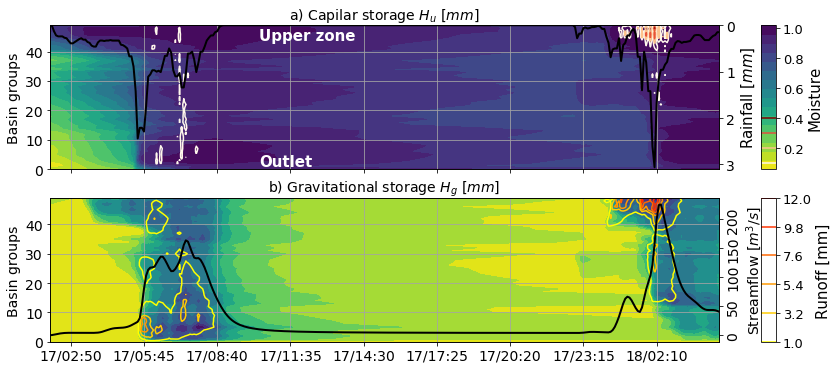
\includegraphics[width=12cm]{figuras/Evolucion_humedad.png}
 \caption{Spatiotemporal analysis of soil moisture variations during events 1 and 2.  a) presents simulated capillary moisture (colored) and returned flux occurrence (white to red regions).  Moisture corresponds to the color bar, and lines to values of returned flux.  In the second Y-axis mean rainfall is shown. b) Presents the simulated gravitational moisture (colored) and the runoff (contour of yellow to red regions).  Additionally, the second $Y$ axis shows the streamflow at the outlet.  Gravitational water content is referenced to color bar of \textbf{a}, runoff values are presented in the color bar of \textbf{b}.}
    \label{fig:HumedadSpatioTemporal}
\end{figure}

\subsection{Soil moisture role}

Figure \ref{fig:SimStreamflow}a presents flux and rain type separations.   Yellow and green lines correspond to convective and stratiform separation.  On the other hand, blue continuous and dashed lines correspond to runoff and sub-superficial flow separation respectively.  Convective portion dominates hydrograph formation followed by runoff.  In both events, stratiform water seems to be more related to sub-superficial flux.  Sub-superficial flow describes the event of May 17 (Event 1), and runoff the event of May 18 (Event 2). This behavior could be due to the temporal occurrence of stratiform and convective formations in both events.  Event 1 starts with a prolonged stratiform event.  On the other hand, event 2 is dominated by convective rain.\\

Precedent capillary moisture of the basin is relevant too, and in this case, plays an important role. Figure \ref{fig:SimStreamflow}b presents capillary (purple), runoff (continuous blue) and gravitational (dashed blue) mean storage oscillations.  As expected, runoff storage only is active during storm events. Gravitational storage reacts during events, with associated recessions, reaching values near zero before the event.  On the other hand, event 1 charged capillary storage, which stills charged just before the flash flood event.\\ 

The event 2 seems to be affected by precedent storage conditions, and the occurrence of successive convective cores in the same regions.  Figure \ref{fig:separacionLluvia} presents rainfall categories for  both events.  To get a robust view of affirmation above, we made a spatiotemporal analysis of rainfall and soil storages of the basin.   Basin cell groups analyze the process dynamics.  This separation let analyze storage oscillations with a coherent spatial discretization.  Cells at the same flow distance from the outlet form a cell group.  For example cells with a distance between 1 and 5 $km,$ are a group.  Figure \ref{fig:ExplainationGroups} presents the examples for 10 groups (left) and for 50 groups (right).  Figure \ref{fig:HumedadSpatioTemporal}a and b presents results obtained for 50 groups. In Figure \ref{fig:HumedadSpatioTemporal}a capillary storage (colored contour), return flux (lines contour) and mean rainfall (black line) are presented.  We present gravitational storage (colored contour), runoff (lines contour) and outlet streamflow at Figure \ref{fig:HumedadSpatioTemporal}b .\\

\begin{figure}[t]
\centering
 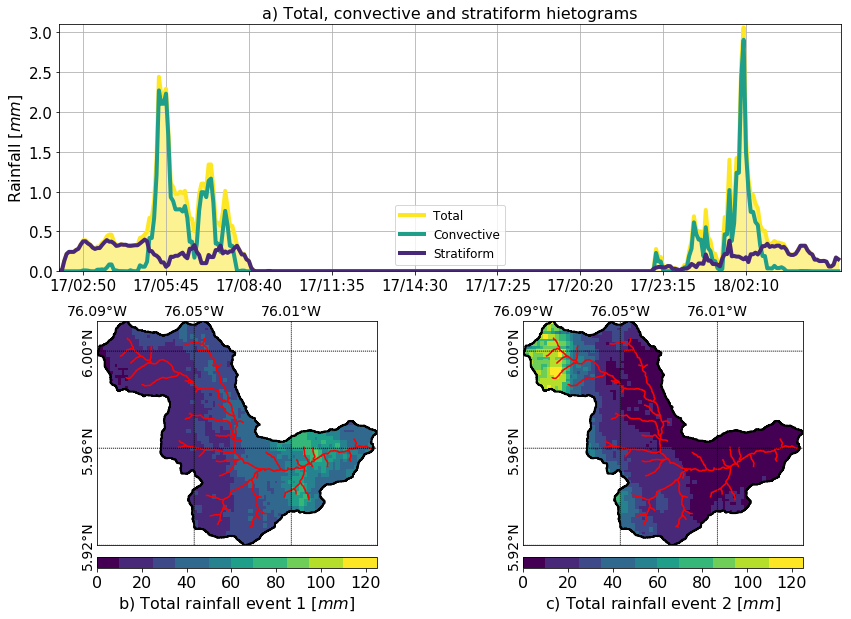
\includegraphics[width=8.3cm]{figuras/Rainfall_separation.png}
 \caption{Mean rainfall (black) and separated participation of convective (Blue) and stratiform (Green) rain in       Liboriana basin, hietogram corresponding to one day before and the analyzed event.}
    \label{fig:separacionLluvia}
\end{figure}

Event 1 and 2 presents relevant processes differences. During event 1 rainfall is distributed in the basin area. Due to this, both gravitational and capillary tanks got charged across the basin. In the event 1, return flux is low, and runoff barely happens near the outlet of the basin.  In the time lapse between both events, there is a recession in the capillary and gravitational storages. Capillary storage decays slower than gravitational, being slower in the upper region of the basin.  Event 2 (flash flood event) starts at 11:00 p.m. in the top part of the basin.  During this event, two convective impulses occur, one at 12:00 p.m. and the other at 2:00 a.m.  (see Figure \ref{fig:separacionLluvia}). The first pulse saturates both storages and produces some return flux and consecutive runoff at the upper region.  Due to soil saturation, the second impulse was transformed mainly into runoff.\\   

\subsection{Rainfall structure role}

Rainfall temporal accumulation has an essential effect on the hydrograph formation. Additionally, the kind of rain accumulation also presents an affection over the hydrograph.  During event 1 rainfall accumulates at a relatively stable rate.  And is the same behavior for convective and stratiform rainfall (Figure \ref{fig:lluviaElapsedCaudal}a).  On the other hand, event 2 presents a significant increase of rainfall rate near the half of the event.  This change in the rain temporal pattern seems to be due to a change in the convective portion (Figure \ref{fig:lluviaElapsedCaudal}b).  In both cases, streamflow and runoff accumulations describe mean rainfall temporal changes.\\ 

Between both events, there is an important change in the elapsed time of the rainfall and streamflow increment. Taking into account time differences in the gray band presented at Figure \ref{fig:lluviaElapsedCaudal}a and b.  For the event 1 the median value of elapsed time ($Et_{p50}$) is 1.12 hours. During the event 2, the same value is 0.79 hours.  Runoff streamflow portion and convective rainfall median elapsed time ($Etc_{p50}$) decrease to 0.42 in the event 2.  Runoff and convective min value of elapsed time ($Et_{min}$) happens near 2:30 hours from the beginning of the event, with a value of 0.25 hours (Figure \ref{fig:lluviaElapsedCaudal}b.  In general  $Etc_{p50}$ and $Et_{min}$ presents a decrease during the event 2.  On the other hand, the elapsed time from stratiform rainfall $Ets$ is stable during both events (see Figures \ref{fig:lluviaElapsedCaudal}a and b).  The occurrence of $Etc_{min}$ is related to the time of which the soil gets saturated, and return flux starts (Figures \ref{fig:HumedadSpatioTemporal}a and b ).  From this point, both convective and runoff accumulation curves present a similar evolution (Figure \ref{fig:lluviaElapsedCaudal}b).\\ 

\begin{figure}[t]
\centering
 \includegraphics[width=8.3cm]{figuras/Elapsed.png}
 \caption{Accumulated rainfall and streamflow for a) precedent event and b) flash flood event. The time scale is $5min$, accumulation is expressed in percentage respect to the total variable value. Median elapsed time ($Et_{p50}$) and minimum elapsed time ($Et_{min}$) are estimated between convective rainfall and runoff portion of streamflow.  Gray bands correspond to the periods taken into account for $Et_{p50}$ and $Et_{min}$.}
    \label{fig:lluviaElapsedCaudal}
\end{figure}

Hydrograph formation is not only determined by the rainfall accumulation or maximum intensity, but also by its structure. Rainfall accumulation was 46$mm$ and 39$mm$ for event 1 and event 2 respectively.  Maximum intensities in both events are similar, 150$mm/h$ and 180$mm/h$ respectively.   Despite this, the precedent event did not produce the hydrograph produced during the flash flood event. Antecedent conditions and precipitation structure possibly produce the differences between both hydrographs.  We discuss precedent conditions in the previous subsection. During the precedent event, convective and stratiform portions present accumulations at the outlet, of 28 and 17 $mm$ respectively (Figure \ref{fig:RainAcumByReach}a). In the other hand, flash flood event accumulate 23$mm$ of convective and 14$mm$ of stratiform rainfall (Figure \ref{fig:RainAcumByReach}b).   According to this, the explanation isn't only in the portions of convective or stratiform rainfall.\\   

Organization of rainfall structure respect to watershed network structure could imply a condition on the hydrological response. This without ignoring the role of precedent soil moisture.   During event 1, convective and stratiform rainfall presents similar accumulation at different watershed scales. Figures \ref{fig:RainAcumByReach}a and c presents these increases. In small sub-basins convective rainfall present higher variations. On the other hand, during event 2, convective accumulation reach higher values for small and medium sub-basins (Figures \ref{fig:RainAcumByReach}b and d).   Convective rainfall tends to cover less area, and at the same time presents an erratic behavior \citep{Steiner1995, Houze1989}.   Due to this, convective accumulation presents higher variations at smalls and sub-basin scales.  Convective occurrence at the upper sub-basins could present major implications, this due to geomorphological and flow accumulation conditions.  This analysis takes two events, an analysis of more events and scales may obtain robust conclusions in this direction.\\

\begin{figure}[t]
\centering
 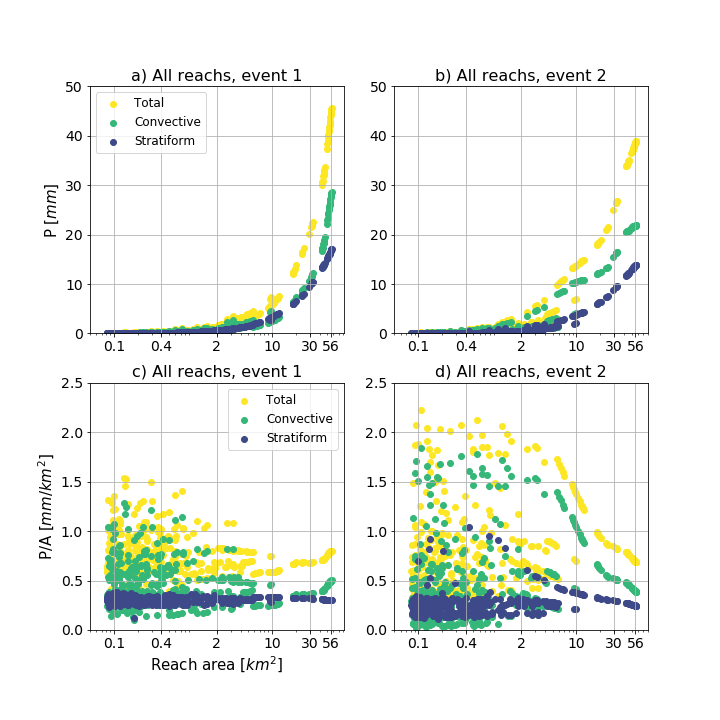
\includegraphics[width=8.3cm]{figuras/RainAcum_by_reach.png}
 \caption{Accumulated rainfall vs. the area at each reach of the basin (logarithmic), yellow dotes correspond to the total rainfall, green to convective and blue to stratiform. Figures a and b correspond to the analysis done for all the reaches in events 1 and 2 (flash flood). Figures c and d correspond to a zoom done for areas below 8$km^2$.}
    \label{fig:RainAcumByReach}
\end{figure}

Convective and stratiform portions could influence the runoff and sub-superficial flow separation.  Additionally, this influence can change across watershed scales.  As shown in Figure \ref{fig:RainAcumByReach}, convective and stratiform accumulation change behavior and magnitude in function of the scale.   This changes must affect fluxes participation.  Figure \ref{fig:PearsonCorr} presents Pearson correlations between the convective and stratiform hydrograph portions with the runoff and the sub-superficial flow hydrograph portions. According to this, rainfall separation has lower relationships with fluxes at small scales (under 5$km^2$).  This could be associated with increasing variability of the hydrograph formation at small scales \citep{Ayalew2014}.  On the other hand, correlations tend to grow with the area, indicating stabilization of the hydrograph formation.\\ 
    
\begin{figure}[t]
\centering
 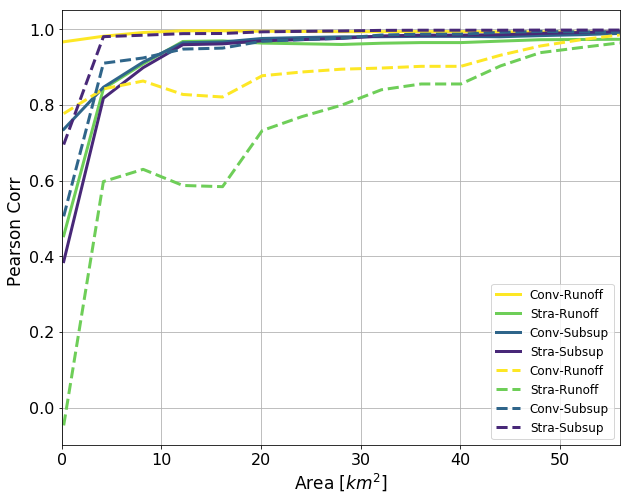
\includegraphics[width=8.3cm]{figuras/CorrPearson_TipoRain_Fluxes.png}
 \caption{Parson correlations for convective and stratiform portions with runoff and sub superficial flow portions at different reaches areas. Dashed lines correspond to precedent event (17/05/2015), continuous lines correspond to flash flood event (18/05/2015).}
    \label{fig:PearsonCorr}
\end{figure}

Apart from the influence of the scale, there are differences between the two analyzed events. In the event 1 (marked with dashed lines), correlations tend to be lower than in event 2.  Additionally, sub-superficial flow presents higher relationships at event 1. While runoff has a high correlation at event 2, this at multiple scales.  Sub-superficial flow relevance is possibly due to the rainfall characteristics during the precedent event, with low intensities and high rates of basin recharge (see Figure \ref{fig:SimStreamflow}b).  On the other hand, saturation process, and a wet soil profile could explain observed higher correlations.  We presume that old water plays a vital role in sub-superficial flow correlations.  Rainfall organization respect to watershed structure could have implications too in this results.\\   

\begin{figure}[t!]
\centering
 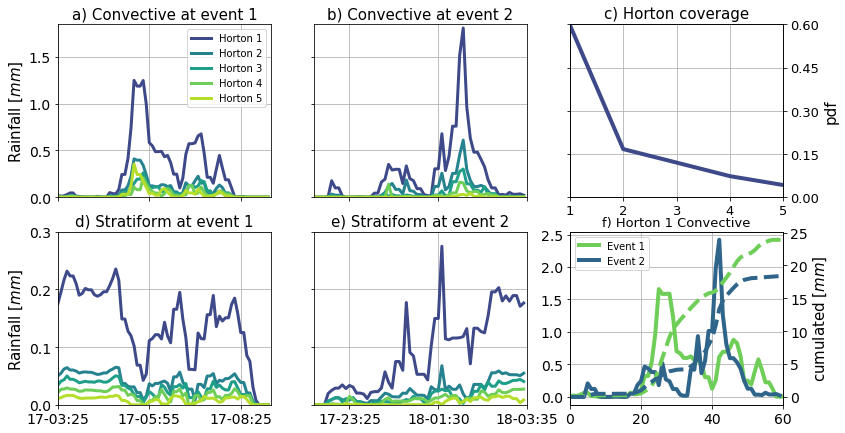
\includegraphics[width=12cm]{figuras/Horton_vs_ConvStrat.png}
 \caption{Mean convective and stratiform rainfall time variation respect to order.  a) and b),  Convective rainfall for events 1 (17/05/2015) and 2 (18/05/2015). d) and e), stratiform rainfall for events 1 and 2. c) percentage of area covered by sub-basins of orders from 1 to 5. f) Comparison of convective portions at orders 1 and 2 sub-basins.}
    \label{fig:HortonVSConvStra}
\end{figure}

\subsection{Floods and Slides Simulations}

Additional to hydrological conditions and fluxes variability, associated risks are modeled and discussed.  Analyzed results correspond to the models coupled to the hydrological model.  We present and discuss the results of shallow landslide model and 1D hydraulic model.\\

\subsubsection{Shallow land slides model implementation}

Landslides model requires additional information about the soil, which is: soil depth ($Z$), cohesion $C'$, friction angle $\phi$ and specific weight $\gamma$.  There is no map with this information; soils information correspond to the description of \citet{Osorio2008}.  It is a clay-slime soil.  According to this description $C'$ is assumed equal to 4$KN$, $\phi$ to 30$^0$ and $\gamma$ to 18, $Z$ vary with the slope according to Table \ref{tab:suelos}. In the landslide model $Z$ map is escalated by a coefficient of 3.5, this is a calibration parameter.  We perform a sensibility analysis over the soils parameters.  Making small variations that oscillate between described values. $\phi$ vary between 25 and 32, $\gamma$ between 17 and 19, and $C'$ between 3.5 and 4.2.  Variations do not produce relevant changes in the results. On the other hand, slight variations in the parameter that scale $Z$ produce significant changes in the model. Such as overestimation of unstable cells, or no unstable cells at all.  Figure \ref{fig:SlidesComparison}a presents the obtained map of total unstable cells at the end of the simulation period. Figure \ref{fig:SlidesComparison}b presents the comparison with observed slides.\\  

\begin{figure}[t!]
\centering
 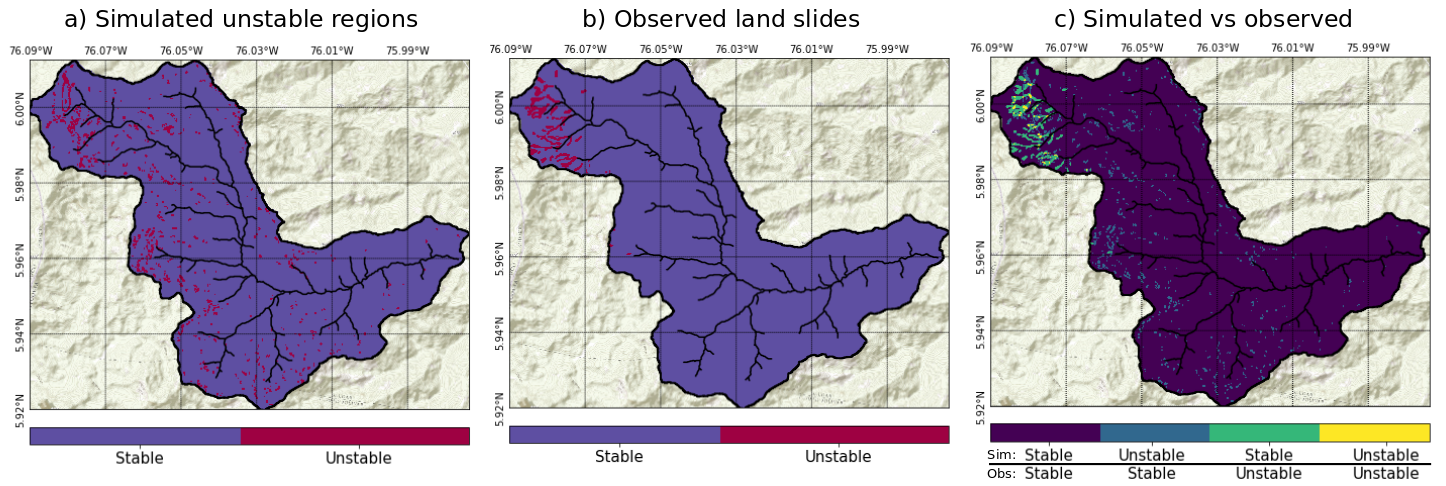
\includegraphics[width=12cm]{figuras/Slides_Simulation.png}
 \caption{Shallow landslide simulation result map. a) Accumulation of estimated unstable (yellow) and stable cells (purple) at the end of the simulation period. b) Comparison with observed landslides, cells marked as purple correspond to a true negative, blue false negatives, green to true negative and yellow to true positive.}
    \label{fig:SlidesComparison}
\end{figure}

\begin{figure}[t]
\centering
 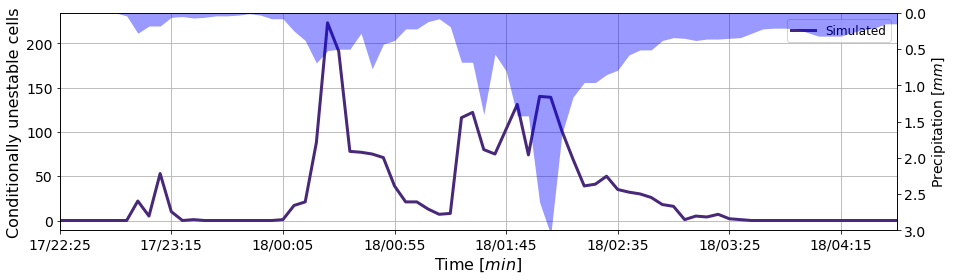
\includegraphics[width=8.3cm]{figuras/Slides_Serie.png}
 \caption{Time series of the number of cells that are considered by the model during the storm event of 18-05-2015, continuous blue line corresponds to the amount of estimated unstable cells in each simulation time, inverse filled graph correspond to the mean rainfall.}
    \label{fig:UnstableCellsSerie}
\end{figure}

Calibration of the landslides model was done searching the maximum overlap between simulated and observed unstable and stable cells (98\% of the total cells). Also reducing false positives and true negatives.   Despite the efforts done in calibration, the total number of cells that are true positives is relatively low. Exact guess of cells by the model in this type of phenomena is considered a hard task \citep{Aristizabal2016, Dhakal2004, Wu1995}. Due to the small temporal and spatial scale at which this process takes place. Additionally, the lack of information increase uncertainty.  Otherwise, the model achieves to represent well the regions that are prone to present shallow landslides. It by showing a significant density of unstable cells in the areas where slides took place (see Figure \ref{fig:SlidesComparison}a and b).\\

According to the model, an essential portion of the landslides happen before the peak of intensity  (see Figure \ref{fig:UnstableCellsSerie}).  Due to the high soil moisture, cells located in the upper region where prone to fail.  Rainfall peak between 00:05 A.M. and 00:55 A.M. detonate slides in the upper area.  Additionally, there is an increase of the soil moisture in the same region. In addition to this soil moisture, convective rainfall peak occurred between 1:20 and 2:15 A.M. and detonated another portion of slides.  During storm events, shallow landslides become a significant source of gravels and sediments.  These particles tend to reach the stream network, increasing the magnitude of the streamflow.  Despite this, there is no explicit link between the landslides model and the hydraulic model.  Nonetheless, the hydraulic model assumes that sediment transport is limited by channel capacity, not by hillslope supply.  It is possible that the sediments from the landslides reach the channel and increase the streamflow during the flashflood.\\ 

\subsubsection{Flash flood spots simulation}

Liboriana is an Andean mountainous basin. In which both, streams and hills present steep slopes. Additionally, the basin presents significant altitude differences, at different scales.  These differences happen from the outlet to the highest peak (Table \ref{tab:geomorfologia}) and inside some of the sub-basins (Figure \ref{fig:Ubicacion}).  Due to this characteristics, there is an important potential energy that increases water transit speed. According to Figure \ref{fig:SectionsMorphology} slopes are higher for order 1 and 2 sub-basins (hills) and channels.  Then slopes descend gradually with increasing order.  At order 1 and 2 hills, water tends to reach faster the channels and slides are prone to occur over this sub-basins. At the same time, there is more sediment production and transport.  Order 3 sub-basins probably act as transport elements, with no important energy losses. At order 4 and 5 sub-basins, floods tend to happen, this due to the widening of the channel  (Figure \ref{fig:SectionsMorphology}f), and loss of slope.\\   

Rainfall tends to fall at order 1 sub-basins, this due to a major area coverage (Figure \ref{fig:HortonVSConvStra}c). Order 1 sub-basins have steep slopes that increase flow speed.  During precedent event and flash flood event, an important portion of the rainfall happen at order 1 sub-basins (Figures \ref{fig:HortonVSConvStra}a and b).  With a major accumulation of convective rainfall in event 1 (Figure \ref{fig:HortonVSConvStra}f). But at the same time more disperse in time and space (Figures \ref{fig:HortonVSConvStra}f and \ref{fig:HumedadSpatioTemporal}a, b).  On the other hand, convective rainfall reaches higher values during event  2 (Figure \ref{fig:HortonVSConvStra}f).\\

\begin{figure}[t]
\centering
 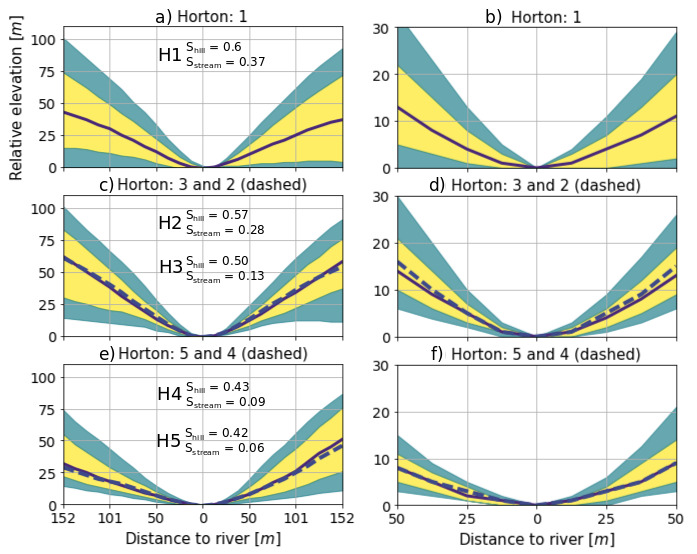
\includegraphics[width=8.3cm]{figuras/Histograma_perfiles.png}
 \caption{Statistical variations of automated extracted cross sections over the stream network, represented by Horton order.  Green bands correspond to percentiles 10-90, yellow to 25-75, continuous and dashed lines correspond to Horton order $\omega_{i-1}$ and $\omega_{i}$ respectively. A, c and e correspond to sections obtained 152m around.  b, d and f are a zoom version took at 50m around.}
    \label{fig:SectionsMorphology}
\end{figure}

Results from the hydraulic model are satisfactory.  Overall results coincide with given description of sections (Figure \ref{fig:SectionsMorphology}).  11\% of flood spots, happen at elements with order 1 and 2.  18, 38 and 32\% happen at orders 3, 4 and 5 respectively.  Additionally, we compare obtained results with observed flood spots.  Although limitations imposed by the DEM used for cross sections, results suggest that the model achieve to make an approximation to the observed flood spots. Obtained results are presented in Figure \ref{fig:SimFloodSpots}.  Results correspond to the time of the peak streamflow at 02:00 A.M on May 18.\\ 

Figures \ref{fig:SimFloodSpots}b to f presents zooms of the results from the outlet to the upper part of the basin respectively. Cases \textbf{e} and \textbf{f} exhibit a satisfactory coincidence with observed flood spots (blue shadow), with failures in specific portions of the stream.  \textbf{c} and \textbf{d} cases present also a good approximation, but with displacements at some points.  Zoom presented in case \textbf{b}  exhibit important differences.  At the entrance of the urban area, the model over-estimate the flood spots.  Additionally, there are some overestimations in the urban area region.  Errors described in Figures \textbf{b}, \textbf{c} and \textbf{d}, could be associated to:  approximations made at the model, maps referencing problems, DEM errors, and differences due to urbanization.  Despite this, results obtained from the model are satisfactory.\\

\begin{figure}[t!]
\centering
 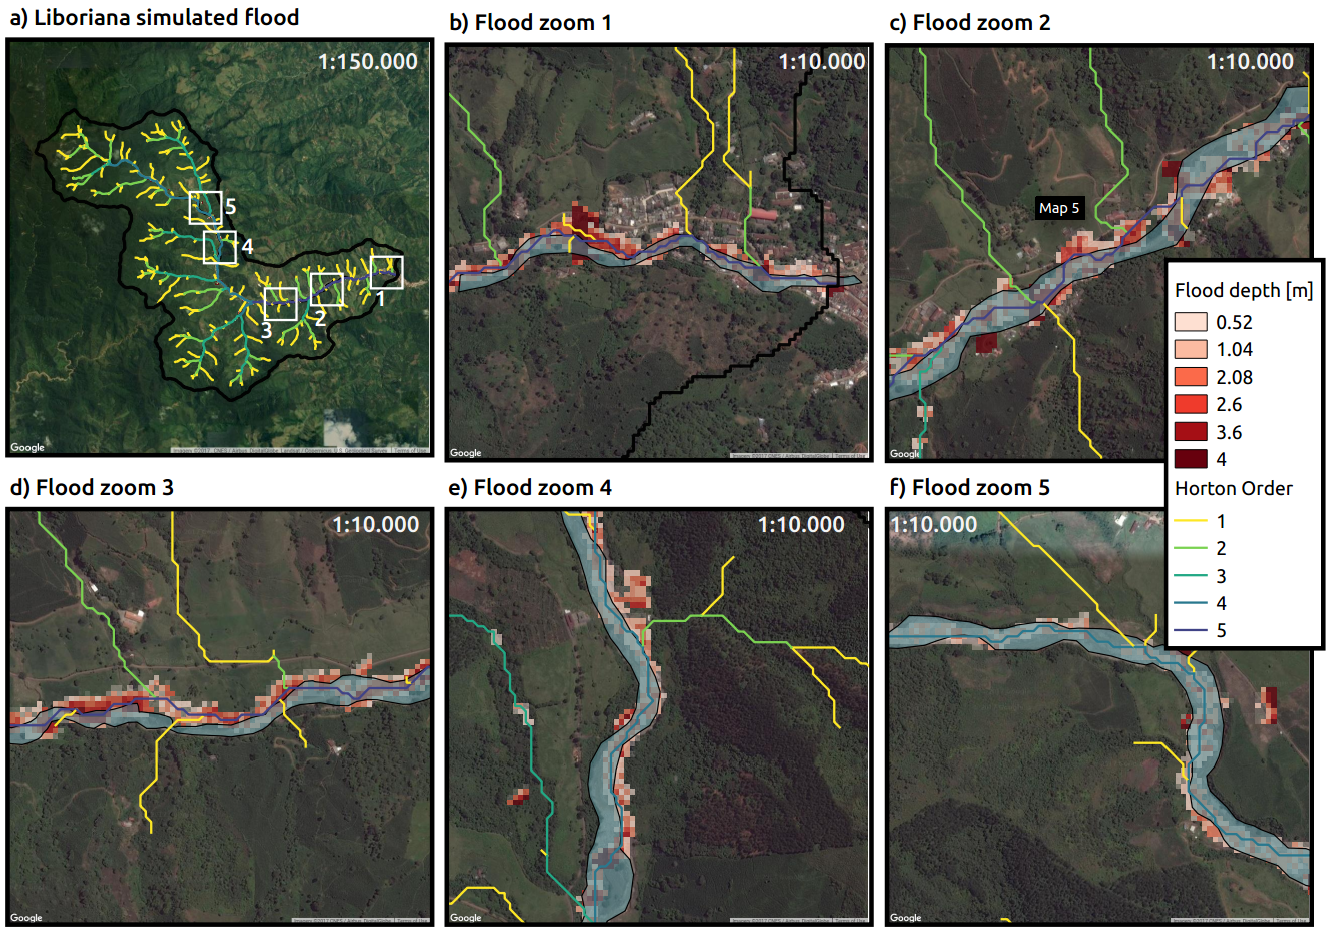
\includegraphics[width=12cm]{figuras/Manchas2.png}
 \caption{Simulated flood spot at the peak of the event 2. a) Complete view of the basin, with zoom regions marked. b) zoom at the outlet of the basin, where an important portion of human and infrastructure happen. c) zoom at la margarita settlement, affected too by the flash flood. d to f: zooms at different parts of the principal stream. They show the adjust of the model (red to white grid) to the observed flood spot (blue polygons).}
    \label{fig:SimFloodSpots}
\end{figure}

The model could include future improvements.  Future work may improve hydraulic parameters such as the width and the diameter of the particles. In the literature exists procedures for parameters regionalization, but they lack validation in tropical regions.  Additionally, the model must have the option to use a detailed DEM, different from the one used for the hydrological model.  We could include several modifications, but, it is essential to keep the model as a tool useful at basins with scarce information.\\

\vspace{5cm}
%%-----------------------------------------------------------
%%-----------------------------------------------------------
%Conclusions
%%-----------------------------------------------------------
%%-----------------------------------------------------------
\section{Conclusions}  %% \conclusions[modified heading if necessary]

During the morning of 18 of May of 2015, a flash flood event happens near 01:00 A.M.  Between 1:30 and 2:30 A.M. the event was reported to local and national authorities. The flash flood left around 120 casualties and significant losses in infrastructure. This paper aims to give a hydrological modeling approach to the processes that took place before and during the morning of May 18 of 2015.  The work seeks to understand the process and to simulate associated natural hazards. For this, we use a highly modified version of SHIA model \citep{Frances2007b}.  Additionally, we add two sub-models.\\  

Hydrological processes have been analyzed using different simulation resources.  The model modification separate runoff and sub superficial flow in the streamflow.  And similarly, to separate convective from the stratiform rain.  Classification of rain fields into convective and stratiform was carried out by using the algorithm proposed by \citet{Steiner1995}.   Additionally, different analysis has been done taking into account the mentioned separations and classifications.\\ 

In addition to the hydrological model, we use two sub-models. The shallow landslide model SHIA-LANDSLIDE \citep{Aristizabal2016}. And the proposed flash flood 1D hydraulic model HydroFlash.  Both models work coupled with the hydrological model.  Landslide model does not achieve to capture precisely slides locations but presents an approximation to vulnerable regions.  On the other hand, HydroFlash gives a close and a satisfactory estimate of observed flood spots.  Results from HydroFlash are part of the model validation.\\    

Flash flood occurrence at Liboriana basin, was influenced by soil moisture conditions and the rainfall structure.  To prove this, we implement the distributed hydrological model at the outlet of the basin.  It is a watershed with limited data, for this, in the calibration we compare the model results with a threshold streamflow.   Hydrological simulations are done from 24 hours before the occurrence of the flash flood.  According to the model, the soil was wet before the start of the event of 18 of May.  Additionally, during the event, three convective impulses happen in the upper region of the basin.  Increasing runoff contribution to the hydrograph formation.\\

In basins like Liboriana, Geomorphology plays an important role.  It is a small watershed with hills that have steep slopes.   A significant portion of described hills, cover the basin.  Additionally, order 1, 2 and 3 tributary channels, tend to present steep slopes.  We suggest more evaluation of those features.  A good approximation to the network-hills structure could give ideas about basins with no information and prone to flash floods.\\

Rainfall structure organization in function of the basin structure could play an important role too.  During the work, we show some results in this direction. With relevant results despite the lack of information, and the number of evaluated events.  Convective cores tend to cover small flat areas.  Their accumulation on sub-basins tends to be erratic but seems to be one of the variables that affect basins like this.  Future work could go in this direction, with expected results that benefit not only hydrological understanding but also risk management.\\ 


% \appendix
% \section{}    %% Appendix A

% \subsection{}                               %% Appendix A1, A2, etc.




\section{Acknowledgements}
The authors want to acknowledge to SIATA and AMVA, for their economical and data support.    

